%!TEX root = da-screen.tex

FIXME: No deterministic symmetry breaking in anonymous networks. Linial's lower bound.

FIXME:

In the previous chapter, we have seen examples of problems that can be solved with a distributed algorithm in the port-numbering model. However, there are many problems that cannot be solved.

As a very simple example, let $N = (V,P,p)$ be a port-numbered network with two nodes, $u$ and $v$, that are connected to each other:
\begin{center}
    \includegraphics[page=\PPnnTwoNode]{figs.pdf}
\end{center}
Assume that we are given a labelling $f(u) = f(v) = 0$. Now let $A$ be any distributed algorithm, and consider the execution of $A$ on $(N,f)$. As the local inputs of $u$ and $v$ are identical, we will have $x_0(u) = x_0(v)$ after the initialisation, that is, nodes $u$ and $v$ have \emph{identical states before round $1$}. It follows that the message sent by $u$ to $v$ in round $1$ is the same as the message sent by $v$ to $u$ in round $1$. Therefore we will have $x_1(u) = x_1(v)$, that is, nodes $u$ and $v$ have \emph{identical states after round $1$}. By induction, we have $x_t(u) = x_t(v)$ for any round $t$. In particular, if $A$ stops in time $T$, we will have $x_T(u) = x_T(v)$, i.e., both $u$ and $v$ produce the same local output.

This reasoning already shows that $A$ cannot produce a proper colouring, a maximal independent set, a minimum vertex cover, etc.\mydash in each of these cases nodes $u$ and $v$ would have to produce distinct outputs. We generalise this observation in Chapter~\ref{ch:covering-map}, when we introduce a very useful graph-theoretic tool, covering maps.

There are also many problems that can be solved with a distributed algorithm, but it requires a lot of time. Techniques that are useful in proving time lower bounds will be introduced in Chapter~\ref{ch:local-neighbourhoods}.
